\documentclass[a4paper, 12pt]{article}

\usepackage{geometry}
\usepackage[figuresleft]{rotating}
\usepackage{hyperref}
\usepackage{pgfgantt}
\usepackage[utf8]{inputenc}
% Bibliography packages and ressources
\usepackage[backend=biber,style=alphabetic]{biblatex}
\addbibresource{1stISIMACheckpoint.bib}
% Appendix packages and figures managments
\usepackage{chngcntr} 
\usepackage{appendix}
% Glossary packages
\usepackage[acronym,toc]{glossaries}

\geometry{hmargin=2.5cm, lmargin=3cm, rmargin=2cm}
\pagestyle{headings}

\title{Notes and Logbook}
\author{Sinan DAROUKH}
\date{4th May 2019}

% =========================================
%               Glossary entries
% =========================================
\makeglossaries

\newglossaryentry{latex}{name={latex},description={Is a mark up language specially suited for scientific documents}}
\newglossaryentry{maths}{name={mathematics},description={Mathematics is what mathematicians do}}

\newacronym{gcd}{GCD}{Greatest Common Divisor}

% =========================================

\begin{document}


% =========================================
%               Title Page
% =========================================
\begin{titlepage}
\maketitle
\end{titlepage}
% =========================================


\renewcommand{\contentsname}{Table of contents}
\tableofcontents
\newpage
\renewcommand{\listfigurename}{Table of figures and illustrations}
\listoffigures
\newpage



\newpage
\section{Internship context}
\subsection{The CERN}
\paragraph{}
The Frenchman Louis de Broglie, who was awarded the Nobel Prize in physics in 1929, was behind the creation of CERN. 
In 1949, he proposed the creation of a European scientific laboratory in order to breathe new life into scientific research following the Second World War. 
In 1952, with the support of UNESCO, the European Council, with the support of the United Nations Educational, Scientific and Cultural Organization (UNESCO), decided to set up a European scientific laboratory for Nuclear Research (CERN), it is the result of an agreement between eleven European governments. 
The municipality of Meyrin, located near Geneva, was chosen to host this laboratory.
In 1954, the first construction work on the site began and on the 29 of September the CERN Convention was signed by twelve European States. 
It was at this date when the research centre, then called the European Organisation for Nuclear Research, was officially established.
\paragraph{}
Today CERN is very well known thanks to its experiences and more particularly its particle accelerator. 
However, it should be noted that many accelerators have succeeded one another on the laboratory site. 
The first was the Synchro-Cyclotron a protons inaugurated in 1957. The accelerators being larger and larger, an agreement was made with France in 1965 to expand the site on French territory. 
Then in 1981 it was decided to build an accelerator in a tunnel with a circumference of 27 kilometers located 100 meters deep underground. 
This tunnel, which is housed in first the LEP (Large Electron Positron Collider). This one was replaced by the current LHC (Large Hadron Collider) in 2008. 
CERN now has 23 member countries and around 2,500 employees and more of 17,500 researchers who come to the Meyrin site to carry out experiments on the premises of the research centre. 
The budget of such an organisation amounts to more than 1 billion Swiss Francs per year.
This funding is fully covered by the Member States.

\subsection{The LHC - Powerful particle accelerator}
\paragraph{}
The LHC, or Large Hadron Collider, is the most powerful particle accelerator in the world built to date. 
It is the last link in a huge particle accelerator complex, which accelerates protons or heavy ions such as lead and creates collisions. 
Particles in the LHC reach a speed of 99.9999991\% the speed of light. 
The collisions take place at four points on the accelerator where the four LHC experiments are located: ALICE, ATLAS, CMS and LHCb.

\subsection{The LHCb Experiment and Internship goals}
\paragraph{}
I am currently working at the LHCb experiment departement which is one of experiment of the LHC.
The main goal of my internship is to streamline the connection process to the monitoring system. 
Actually the LHCb departement use multiples ssh connection to monitor the experiment and its results. 
In order to simplify this workflow, I have been investigating on special components on WinCC-OA to set up pre-existing project online.

\section{Technologies}
\subsection{What is WinCC-OA ?}
\paragraph{}
SIMATIC WinCC is a Supervisory Control And Data Acquisition (aka SCADA) and human-machine interface from Siemens. 
SCADA systems are used to monitor and control physical processes involved in industry and infrastructure on a large scale and over long distances. 
SIMATIC WinCC can be used in combination with Siemens controllers. 
WinCC is written for the Microsoft Windows operating system, but it could be use on Linux operating system. 
WinCC-OA aims are mainly to control and acquire data from the sensors from reals controls on experiments.
You may have heard about PVSS, it was a SCADA system, made by ETM. 
Siemens now owns ETM and rebranded PVSS as WinCC-OA, but it's still the same tool. 
It's a tool for building SCADA applications. WinCC-OA is the SCADA system chosen by JCOP (CERN).

\subsection{What is JCOP ?}
\paragraph{}
JCOP stands for Joint COntrols Project which is a collaboration between the LHC experiments, the PH Departement and EN-ICE, the Controls Group in the Engineering Departement. 
JCOP aims to reduce the overall manpower cost required to produce and run the experiment control systems.
The JCOP Framework provides all the components required for WinCC-OA tool. 
Basically, it's a layer of software components and shared tools that might be useful for modelling LHC Experiment.

Around the end of 1997, a common project, the Joint Controls Project (JCOP), was setup between the four LHC experiments and a Controls group at CERN, to define a common architecture and a framework to be used by the experiments in order to build their Detector Control Systems (DCS).
The JCOP Framework adopted a hierarchical and highly distributed architecture providing for the integration of the various components in a coherent and uniform manner. 
The Framework was implemented based on a SCADA (Supervisory Control And Data Acquisition) system called WinCC-OA (formerly PVSSII). 
While WinCC-OA offers most of the needed features to implement a large control system, it was felt that a tool for implementing higher-level logical behavior was missing.
For this reason, the JCOP project was complemented by the integration of SMI++; a toolkit for sequencing and automating large distributed control systems, whose methodology combines three concepts: object orientation, Finite State Machines (FSM) and rule-based reasoning.

\subsection{HTTP Server - Addons}
The HTTP Server integrates Internet technologies directly into WinCC OA. Implemented as an add-on for the Control Manager, possible applications are many and diverse. 
The HTTP Server can be used as a web server for static HTML pages including download facility or to generate dynamic HTML pages. 
This allows you to make data from WinCC OA available to many users at the same time. The complete WinCC OA programming language Control is thus available for server-side scripting tasks.
\paragraph{Advantages of the HTTP Server :}
\begin{itemize}
    \item Provide custom HTML pages incorporating data from WinCC OA for intranet / Internet.
    \item WEB alert screen with acknowledge function and free choice of filters.
    \item Diagnostics page displaying hard disk capacity, RAM, processor usage, alert \\throughput, users logged in and more.
    \item "HTML references" allow you to replace \$parameters at runtime without any special knowledge of HTML, that is, you can query any data points through the Internet.
    \item Querying WinCC OA data using SQL
    \item Transfer static HTML pages
    \item File transfer (HTTP download).
    \item HTTP Server uses WinCC OA specific tags in HTML.
\end{itemize}

\subsection{ULC UX - Addons}
The ULC UX is a User Interface client for WinCC OA based on the VNC technology and HTML5 technology. 
It is used as a new alternative to the WinCC OA UI (native UI on Windows and Linux) and the WinCC OA Web Client (Plug-in-based web solution).
The ULC UX can use already engineered panels without any special adaptions, and it provides a very high compatibility to the native UI functionality

\paragraph{Benefits :}
The ULC UX combines following benefits in a single UI solution:
\begin{itemize}
    \item No installation is required on client side
    \item Communication is secured by using SSL encryption
    \item User management can be performed by using SSO
    \item Usage of WinCC OA panels without changes to the existing control scripts
\end{itemize}
\paragraph{Performance Requirements : }
There are parameters which have an influence on the performance of the ULC UX in the web browser.
\begin{itemize}
    \item Bandwidth
    \item Latency
    \item Dynamic panel content
    \item CPU performance of the web server
    \item Available memory on the web server
\end{itemize}
Because the performance and the possible ULC UX connection to one web server are highly addicted to the panel and the scripting inside the panel we cannot guaranty any fixed number of possible connections. 
This will be highly customer panel dependent and the customer will need to test his own panels to get a possible ULC UX connection. If the performance of one web server is not sufficient load balancing can be used with multiple web servers.
\paragraph{Architecture}
The basic architecture displayed in the figure below gives an overview for the involved WinCC OA managers or software modules for the WinCC OA ULC UX.
\begin{figure}[!ht]
    \centering
    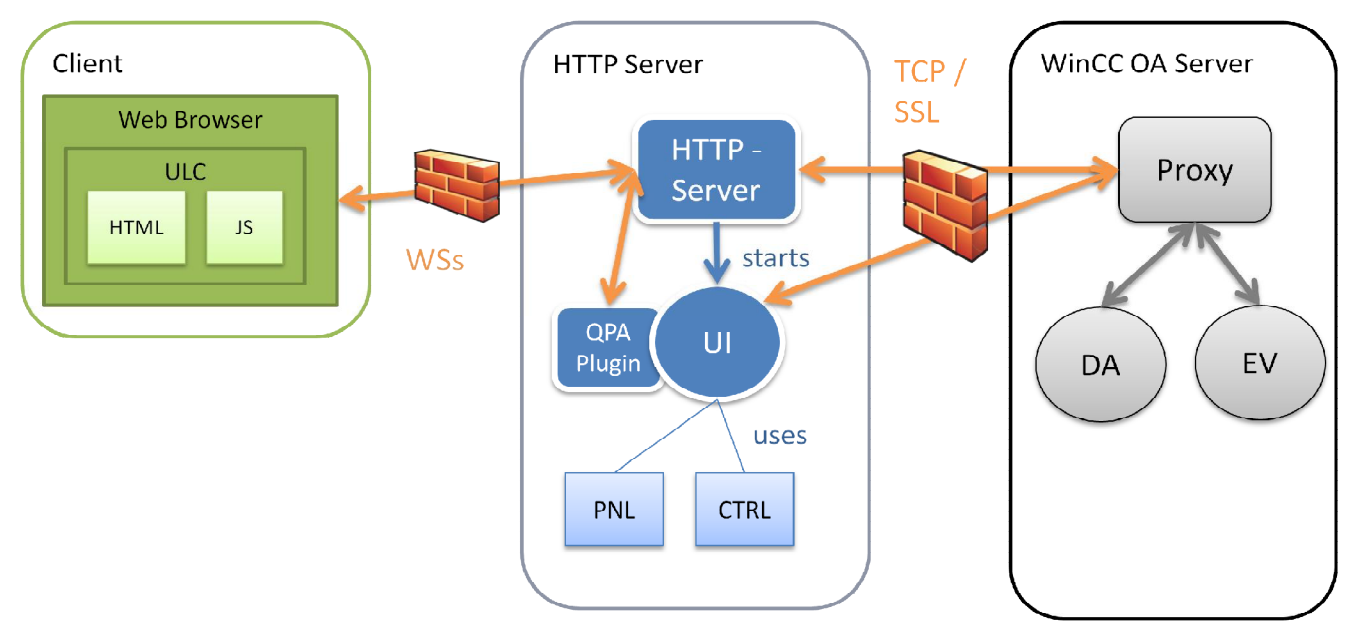
\includegraphics[scale = 0.4]{images/ulc_ux_architecture.png}
    \caption{ULC UX Architecture}
\end{figure}\newline
When a browser tries to connect to the ULC UX - URL of the WinCC OA HTTP Server, the HTTP server returns the ULC UX web page and automatically starts a local WinCC OA UI manager. This server side UI manger transfers displayed information of the UI into HTML 5 interpretable data chunks.. A Java Script library at Client side afterwards interprets those data chunks and draws the graphics in the browser.

\clearpage
\glsaddall
\printglossaries

% =========================================
%               Appendices
% =========================================
\counterwithin{figure}{section} % Figures counters reinitialised
\newpage
\appendixpage
\begin{appendix}
    \section{Logbook}
    \subsection{Iteration from Monday 4th May to Friday 15th May}
    \paragraph{Objectives of the iteration :} 
    The main goal of this iteration was to get more familiar with WinCC-OA and the JCOP Framework. 
    Also the main idea was to think about how to make the LHCb experiments monitor more accessible from the web without changing the WinCC-OA pre-existing project drastically.
    \paragraph{Tasks done \& notes :}
    \begin{itemize}
        \item Reading documentations about WinCC-OA.
        \item Setting up the main project.
        \item Reading/Writting emails to the ISIMA supervisor (Mr HILL) and the CERN one (Mr Luis Granado Cardoso).
        \item Helping and exchanging with Loann, who is working on the same technology as me.
        \item Going through the tutorial slides.
        \item Experimenting through Exercice 1,2,3 and 4.
        \item Facing some difficulties with the CTRL system.
        \item Reading documentation about HttpServer
        \item Watching videos about WinCC-OA on \href{https://www.youtube.com/user/ETM2011}{Siemens} and \href{https://www.youtube.com/channel/UCGBnHd1-B-Zg9MDsjTk0-Sw}{KAASM}'s youtube channel. 
        \item Doing daily meetings with Luis to track the progess.
    \end{itemize}

    \subsection{Iteration from Wednesday 15th May to Sunday 20th May}
    \paragraph{Objectives of the iteration :}
    The aim of this iteration was to look at all the documentation about the WebServer components in WinCC-OA, how to navigate properly between panels, how to manage users access permissions and restrictions, and how to well organise configs files in a project. I was sick during a part of this iteration, so I did not work effictively on Monday
    \paragraph{Task done :}
    \begin{itemize}
        \item Reading all the documentation
    \end{itemize}

    \paragraph{Notes :} 
    I have been reading the documentation about the configuration files :
    \begin{itemize}
        \item config.level is for managers configurations, and basically, loading libs through this file.
        \item config.redu is for redundancy, that we are not seeking for, at the moment
        \item config.http is a premade file from the WinCC-OA folder
        \item config.webclient is an additional file for configuration Desktop and Mobile UI add-ons\dots (Not what we are looking for)
    \end{itemize}
    I have tested multiple stuffs on those. Nothing really can simplify the actual config (root) file.
    I guess there's another option not yet tested which is the own configuration file, I don't know if we can use more than once.\newline
    For the navigation fluidify and simplification issues, I have been testing stuffs and reading about the differences between Modules, Embedded Modules , Child and Root Panel.\newline
    To navigate properly, I think I should take a look at the Topologies panels components... The embedded modules through one root module, may be the best layout option.

    \subsection{Iteration from Wednesday 20th May to Wednesday 27th May}
    \paragraph{Objectives of the iteration :}
    \begin{itemize}
        \item User permissions, one can connect to view, another can connect to administrate
        \item Play with the alarm Screen, make a shortcut to it
        \item (FSM) Implement one, how it goes on the ULC components
    \end{itemize}
    \paragraph{Tasks done :}
    \begin{itemize}
        \item Login panel has been implemented (worked on both ULC and Regular WinCC)
        \item Can access on user admnistration panel through it : Module \textgreater\ SysMgm \textgreater\ Permissions \textgreater\ User Admnistration, which on root access list all users and permissions
        \item Groups \textgreater\ Admnistrate \textgreater\ Permissions : You can change the group permissions but also, create new groups with new permissions
        \item Permissions are logged in an Authorization Bits system. The first five bits are already define, they are predefined and un-changeable, but you can change the description if you want and texts of it : 
        \begin{itemize}
            \item 1 : Visualisation: Visualize only
            \item 2 : Normal operator authorization: permits the opening of child panels.
            \item 3 : Advanced operator authorization: permits execution of commands, explicit setting of replacement values, input of correction values as well as changes to all value range types.
            \item 4 : Administration: permits the use of the PARA.
            \item 5 : Acknowledgement: permits acknowledgment of alerts.
            \item 32 : Allows SSO for one work station
        \end{itemize}
        \item Can also access on login statistics panel to see whose connected : Module \textgreater\  Login Statistics
        \item We can manage the Components access thanks to the boolean getUserPermission() function : CONTROL \textgreater\  Control functions \textgreater\ G \textgreater\ getUserPermission()
        \item We can check on the Main Panel, by Login via Guest or via Root
        \item Auto login done, with inactivity (Glitch with inactivity, security one) (UI number changed some time)
        \item Alarm Panel : I have worked on it, but there is a glitchy features, the windows appears behind the Alarm Screen
        \item I also haven't the time to experiment on the FSM.
    \end{itemize}

    \subsection{Iteration from Wednesday 27th May to Tuesday 2nd June}
    \paragraph{Objectives of the iteration :}
    \begin{itemize}
        \item Adding and testing the FSM, on the Web app, it actually works but... it took me a lot of times.
        \item Create Shortcut for opening differents kinds of panels, I had issues with the DEN Panel... But now it works
        \item Didn't check on the Alarm Screen and the Users Permissions, as I had issues with the DNS part of the tuturials.
    \end{itemize}

    \subsection{Iteration from Thurday 3rd June to Monday 8th June}
    \paragraph{Objectives of the iteration :}
    \begin{itemize}
        \item Look at the documentation about Distribution Manager, Distribution Configs Files, Distributions Systems etc...
        \item Test to implement the following panel : \\ (Location : /localdisk/wincc/prod/["LBECSINFO","ECS"]/panels/)
        \begin{itemize}
            \item lbAlarmHandling/lbAlarmScreen.pnl
            \item FarmUsagePlot.pnl
            \item lbECS/lbOPCMonitor.pnl
            \item lbTriggers/lbTriggersOverview.pnl
            \item lbTrending/lbTrending.pnl
        \end{itemize}
        \item Use the current project as the main client, connected to the ECS and LBECSINFO projects.
    \end{itemize}
    I have read a lot of the documentation about the distributed managements, and distributed systems.
    I have learnt that you can configure them through an existing wizard only if you create a new project.
    Else you should do it via the configuration files. I have tried to launch script from the copied project, but without any success. \newline
    The Test Project configuration file should look like this :\newline
    [general]\newline
    distributed = 1\newline
    [dist]\newline
    distPeer = "dist\_name\_ECS" 1130\newline
    distPeer = "dist\_name\_LBECSINFO" 1140

    \begin{figure}[h]
        \centering
        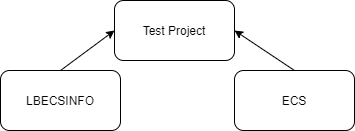
\includegraphics[scale = 0.5]{images/subsystem.png}
        \caption{Example of distributed projetcs}
    \end{figure}

    \subsection{Iteration from Monday 8th June to Wednesday 10th June}
    \paragraph{Objectives of the iteration :}
    The meeting with Luis helped me debugging the and connecting the two distributed projects. I am currently trying to launch differents panels from the ULC web components.
    I have succeed to open them, but... the data point seems to not be well-connected or at least are connected to the wrong project.
    I achieved this by updating the config files, which is I think not the cleanest way to do it, but the fastest (Testing first)
    We can explore two options which are : copying all the project in a special repos, or we can try with the addSymbol() functions, or we can also try to copy all the paths.

    \subsection{Iteration from Friday 12th June to Friday 19th June}
    \paragraph{Objectives of the iteration :}
    Connect all those panels and see if they work properly in the ULC UX components. See panels from iteration 03/06 to 08/06
    \subsection{Iteration from Friday 19th June to Wednesday 24th June}
    \paragraph{Objectives of this iteration :}
    \begin{itemize}
        \item Create a new main page for the app, which should be more similar than the one already in use.
        \item Create shortcuts to the following panels :
        \begin{itemize}
            \item LHCb Top FSM - Without the possibility to click anywhere
            \item LHCb - LHC - Big Brother
            \item Alarms Screen
            \item Trending panels
        \end{itemize}
        \item Also check if we can have to access to other stuffs than WinCC-OA panels onto the ULC UX components.
    \end{itemize}
    \paragraph{Notes :}
    I have issues on displaying both FSM from ECS. Seems that there are missing datapoints. Also, I have noticed some stuffs on the right click event.
    I need to go deep down the code of the Alarm Panel and the Trending one, too see why it's working only if you launch the Alarm panel before.
    I also need to continue on the tools bars.
    \subsection{Iteration from Wednesday 24th June to Thursday 30th June}
    \paragraph{Objectives of this iteration :}
    \begin{itemize}
        \item Continue the investigation and research on the IFrame stuffs.
        \item See if we can fix the right-click issues as I have new hints.
        \item Wait until Luis fix the DP non-exists from the LHCb Top \& BigBrother panels.
        \item Also continue with the tools bars customizations.
    \end{itemize}
    \paragraph{Notes :}
    \paragraph{Investigates :}
    \begin{itemize}
        \item navigation buttons, layout managements
        \item tabs for the layout
    \end{itemize}
    
    For next Thursday 11hOO : 
    - Send HILL contact to Luis - (DONE)
    - LHCb Top / Big Brother to display correctly through personal panel : FSM ui panel
    - FarmUsagePlot -> Luis will use another plot (DONE)
    - Figure out the right click issues on the Trending pnl
    - Polish the look of the panels (DONE)
    - Layout for the WebViewer make this resizeable (DONE)
    - Make button directly goes to the part of web logbook (DONE)
    \newpage
    \section{Real Gantt chart}
    \begin{figure}[h]
        \centering
        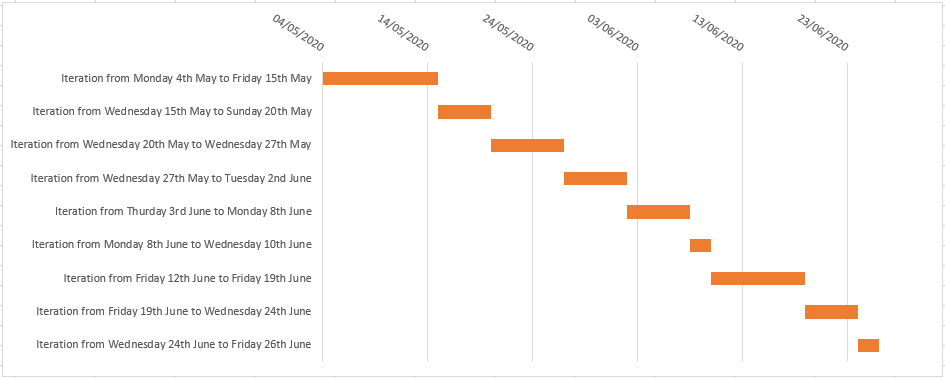
\includegraphics[scale = 0.6]{images/gantt.png}
        \caption{Real Gantt Chart}
    \end{figure}
\end{appendix}

\newpage
\section{References}
\nocite{*}
\printbibliography[heading=subbibintoc,type=article,title={Bibliography}]
\printbibliography[heading=subbibintoc,type=misc,title={Webography}]


\end{document}